\chapter{Local Consistency nei Soft CSP} \label{ch:Local Consistency nei Soft CSP}
\section{Local consistency}
Fare Local consistency nel caso di CSP Soft non significa eliminare dei valori dal dominio, ma significa ridurre (ottimizzare) il valore del semiring associato a quella variabile in maniera tale da fare in modo che questo valore si avvicini il più possibile a quello della soluzione finale.
\subsubsection{Esempio con CSP Soft:}
\begin{figure}[htp]
	\centering
    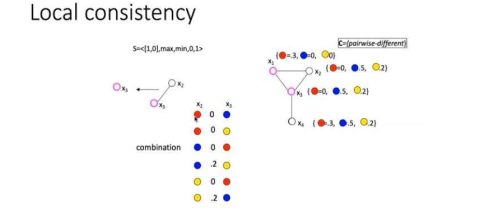
\includegraphics[width=10cm, keepaspectratio]{img/Cap5/LocalConsistency.png}
\end{figure}
In questo esempio sono presenti solo vincoli unari, che mi dice che quando ad $x_1$ gli assegno rosso ha valore 0.3, quando blu o giallo ha valore 0; cosi per tutte le variabili. Siccome il valore 0 è il bottom del semiring, dare 0 significa che non sono assegnamenti permessi, quindi li possiamo direttamente
eliminare.
\\
\textbf{Ottimizzazione della soluzione su CSP Soft: } Voglio ridurre (ottimizzare) il dominio della variabile $x_3$ , vediamo come fare con tutti i passaggi:
\begin{enumerate}
    \item \textbf{Combinazione:} Prendo tutte le possibili tuple, gli assegno un valore e poi in base all'operatore di combinazione (che in questo caso è min) faccio la proiezione.
    \\Quindi parto cosi:
    Il minimo se $x_2$ è rosso e $x_3$ è blu è 0, perchè è il minimo tra 0 e 0.5.
    \\Il minimo se $x_2$ è rosso e $x_3$ è giallo è 0, perchè è il minimo tra 0 e 0.2.
    \\Continuo cosi per tutte le tuple.
    \\Non ho considerato le coppie di colore uguale perchè c'era scritto $pairwise-different$.
    \item \textbf{Proiezione:} Tra tutti i risultati che genera la combinazione faccio la proiezione sulla variabile in questione, in questo caso $x_3$. Adesso: quanto valore ha $x_3$ quando ha valore rosso? Devo fare il massimo tra 0 e 0 che è 0 e tutto rimane invariato perché $x_3$ sul rosso ha comunque 0. Per $x_3$ $=$ blu il massimo è 0.2. Per $x_3$ $=$ giallo il massimo è comunque 0.2. L’unica modifica da apportare quindi è al blu di x3 che al posto di 0.5 ha valore 0.2.
\end{enumerate}
Nel caso \textbf{Crisp CSP} i valori vengono eliminati completamente dal dominio. Nel caso \textbf{Soft CSP} ottimizzo il valore di semiring associato a quell’assegnamento. Una volta ottimizzati tutti i valori si utilizzano tecniche di \textbf{Branch And Bound}, che può essere applicato o all’inizio o durante la ricerca, per trovare la soluzione.
\newpage
\subsection{Esempio con Fuzzy}
\begin{figure}[htp]
	\centering
    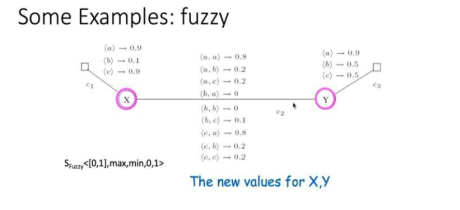
\includegraphics[width=12cm, keepaspectratio]{img/Cap5/Fuzzy.png}
\end{figure}
Consideriamo il vincolo unario c1 sulla variabile X ed il vincolo binario $c_2$ sulle variabili X ed Y. Faccio $c_1$ $(x)$ $c_2$ proiettato $x(a)$:
\begin{enumerate}
    \item Combinazione (Min): $c_1$ combinato $c_2$ ($c_3$ non lo prendo in considerazione perchè faccio $(x$):
    \begin{itemize}
        \item Quando vale $< a, a >?$ Faccio 0.9 min 0.8 $=$ 0.8
        \item Quando vale $< a, b >?$ Faccio 0.9 min 0.2 $=$ 0.2
        \item Quando vale $< a, c >?$ Faccio 0.9 min 0.2 $=$ 0.2
    \end{itemize}
    Facendo questo ho combinato i vincoli c1 e c2 . Per sapere poi quanto vale $c_1$ $(x)$ $c_2$ devo andare a proiettare su X.
    \item Proiezione (Max): Prendo il massimo tra 0.8, 0.2, 0.2. In conclusione, al posto di 0.9 su (a) posso scriverci 0.8.
\end{enumerate}
\textbf{Altra domanda sul fuzzy (assegnamento): } Quanto vale l’assegnamento $x=a$, $y=b$? 
\\devo fare il minimo tra 0.9, 0.2 e 0.5 che sarebbe 0.2. 
\\(Non applico la proiezione quindi non uso il massimo).
\\Altra domanda: Applichiamo local consistency per X $=$ a.
\\Devo fare min(0.9, 0.8, 0.9) $=$ 0.8.
\\Devo fare min(0.9, 0.2, 0.5) $=$ 0.2.
\\Devo fare min(0.9, 0.2, 0.5) $=$ 0.2.
Se vado a proiettare fa 0.8 perchè prendo il massimo. Se io vado a calcolare la soluzione adesso vado a calcolare la soluzione di '' quanto vale x$=$a y$=$b''?
\\min tra 0.8, 0.2 e 0.2 = 0.2 che è come prima, la soluzione non è cambiata.
\textbf{Ho migliorato il bound ma non ho modificato la soluzione, è una cosa buona.}
\\Nell’ esempio successivo (prossima sezione, sarebbe quello probabilistico) la soluzione \textbf{viene modificata} a 0.72 e non più a 0.9 quindi non posso accettarla, è proprio sbagliata.
\section{Idempotenza degli operatori}
Un operatore si dice idempotente se facendo:
\begin{center}
    $a operazione a$ mi restituisce sempre a.
\end{center}
L’idempotenza si può analizzare sia per gli operatori che si usano per la Proiezione sia per quelli di Combinazione.
\\Proiezione sia per quelli di Combinazione.
\begin{itemize}
    \item Idempotenza su \textbf{Combinazione}: Dipende strettamente dal semiring utilizzato:
    \begin{itemize}
        \item \textbf{Fuzzy:} Idempotente, perchè il minimo tra a ed a è sempre a (il minimo tra due valori uguali da sempre lo stesso valore).
        \item \textbf{Probabilistic:} Non idempotente, perchè a $*$ a non fa esattamente a (ad esempio 0.1 $*$ 0.1 $=$ 0.01, la moltiplicazione infatti non ha la proprietà di idempotenza).
        \item \textbf{Weighted:} Non idempotente, perchè a $+$ a non fa esattamente a.
        \item \textbf{Classic:} Idempotente, infatti a and a $=$ a
    \end{itemize}
    \item Idempotenza su \textbf{Proiezione:} Tutti gli operatori sono idempotenti e questo segue dalla definizione stessa di c-semiring (definisco l’ordinamento quando effettuo la proiezione).
\end{itemize}
La distinzione tra operatore idempotente e non idempotente è importante perchè gli algoritmi di consistenza locale solo nel caso in cui la combinazione fosse idempotente \textbf{mantengono le soluzioni del problema}. Qualora facessi arc-consistency su semiring che non ammettono operazioni idempotenti la soluzione che si genera è proprio \textbf{sbagliata}, e non può essere accettata.
\newpage
\textbf{Vediamo un esempio in cui applicare arc-consistency va a modificare la soluzione finale del problema} (e quindi non è accettabile):
\begin{figure}[htp]
	\centering
    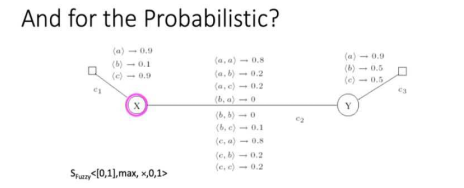
\includegraphics[width=12cm, keepaspectratio]{img/Cap5/probabilistc.png}
\end{figure}
\textbf{Domanda:} Quanto vale l’assegnamento x $=$ a, y $=$ b su questo problema? 
\\devo moltiplicare 0.9, che sarebbe x$=$a, per $<$ x $=$ a, y $=$ b $>$ che sarebbe 0.2 per y $=$ b che sarebbe 0.5. Il risultato è 0.09.
\\Domanda: Quanto vale c1 c2 proiettato x (su a)? devo fare la combinazione:
\begin{itemize}
    \item 0.9 $*$ 0.8 $=$ 0.72
    \item 0.9 $*$ 0.2 $=$ 0.18
    \item 0.9 $*$ 0.2 $=$ 0.18
\end{itemize}
Poi prendo il Massimo (proiezione) che sarebbe 0.72 e questo valore mi va al posto di 0.9. Il problema però è che ho cambiato la soluzione finale, perchè la proiezione mi ritorna proprio il 0.72 che è un valore errato data la non idempotenza della moltiplicazione (è proprio una soluzione sbagliata).

\vspace{0.8cm}

L’operazione di local consistency nei CSP Crisp quindi classici è importante perchè mantiene la soluzione del problema riducendo gli elementi del dominio e non modificando le soluzioni.

\vspace{0.5cm}

Nel caso Soft invece, la soluzione non viene modificata solamente se l’operazione di combinazione è idempotente. Nel caso in cui non lo fosse si andrebbero a modificare le soluzioni stesse del problema, e quest’ultime non sarebbero accettabili perchè sbagliate.
\newpage
\subsection{Altro esempio con vincolo c3}
\begin{figure}[htp]
	\centering
    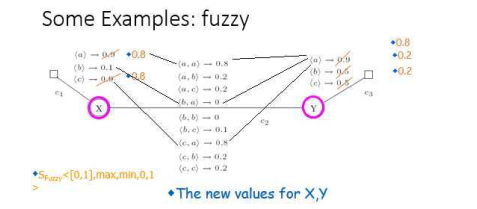
\includegraphics[width=12cm, keepaspectratio]{img/Cap5/fuzzy2.png}
\end{figure}
I nuovi valori per il vincolo c3 sono ottenuti analizzando prima y $=$ a e quindi poi si analizza (a, a) e poi x $=$ a. Poi y $=$ b e quindi poi (b, b) e poi x $=$ b. Utilizzando la combinazione e poi la proiezione i valori tornano quelli.
\subsection{Semiring con operazioni non idempotenti}
\subsubsection{Divisione}
Vogliamo ottimizzare i CSP Soft anche se la loro operazione di combinazione non è idempontente.
\begin{figure}[htp]
	\centering
    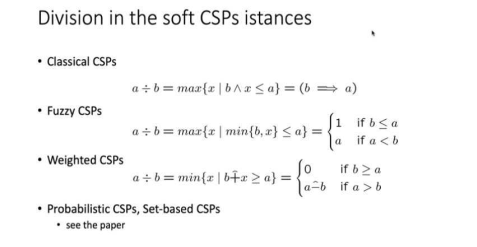
\includegraphics[width=12cm, keepaspectratio]{img/Cap5/DIvisione.png}
\end{figure}
\\L’operatore che utilizzeremo è l’opposto dell’operatore di combinazione ed è chiamato Diviso: $\div$. Analizziamo la riga del Fuzzy:
\begin{itemize}
    \item Prima versione: L’operazione inversa del minimo, indicata con l’operatore $\div$ è max. Supponiamo che l’elemento x sia tale che b $*$ x $=$ a, la domanda è: Quanto fa a $\div$ b? Fa quell’elemento x tale che il minimo tra b ed x è minore uguale di a. Devo quindi in qualche modo andarmi a trovare gli inversi degli operatori visti prima.
    \item  Seconda versione: Quando fa a $\div$ b? (si legge a Diviso b). Fa il numero più grande x tale che il minimo tra b ed x è più piccolo di a
\end{itemize}
Analizziamo la riga del \textbf{Weighted:}
\\Quanto fa a $\div$ b? Fa il più piccolo (min) elemento x tale per cui b $+$ x fa a. Questo però lo possiamo fare solo se a è maggiore di b (altrimenti si prenderebbero in considerazioni valori non consoni tipo negativi) e se b è maggiore uguale di a si da come risultato 0.
\\\textbf{Esempio probabilistico:}
\begin{figure}[htp]
	\centering
    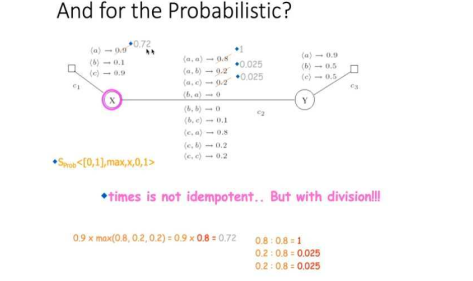
\includegraphics[width=12cm, keepaspectratio]{img/Cap5/Probabilistic2.png}
\end{figure}
Come faccio ad ottimizzare il CSP in maniera tale da mantenere le soluzioni?
\\Inizio in maniera identica al precedente metodo:
\begin{itemize}
    \item Combinazione
    \begin{enumerate}
        \item 0.9 * 0.8 = 0.72
        \item 0.9 * 0.2 = 0.18
        \item 0.9 * 0.2 = 0.18
    \end{enumerate}
    \item Proiezione: Max = 0.72
\end{itemize}
\newpage
Fatto questo devo \textbf{dividere per il massimo valore tra tutti quelli utilizzati:}
\begin{center}
    $max$(0.8, 0.2, 0.2) = 0.8
\end{center}
Ora divido per 0.8 tutti i valori nel vincolo $c_2$ cosi da ottenere i valori in figura. Dato che ho ottimizzato il valore di (a) e cambiato i valori interessati, la soluzione rimane invariata, quindi anche su semiring non idempotenti si può fare arc-consistency grazie all'operatore di Divisione ($\div$).
\begin{center}
    \textbf{Importante}
\end{center}
In questo caso abbiamo utilizzato la divisione perchè era l'operazione inversa della moltiplicazione (che è l’operatore di combinazione utilizzato nei CSP probabilistici). Se però l’operazione di combinazione fosse stata la Somma (e quindi CSP Weighted) l’operazione $\div$ sarebbe stata la sottrazione.